\chapter{Volume Rendering mit 3d-Texturen}
\section{DVT}
\begin{figure}[H]
	\centering
	\begin{subfigure}{.47\textwidth}
		\centering
	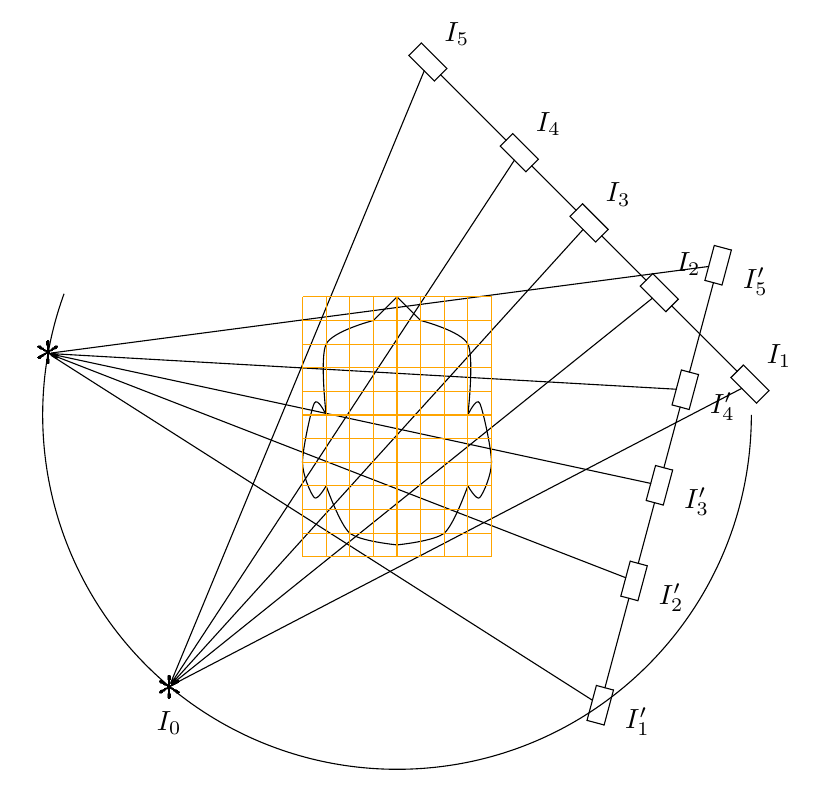
\begin{tikzpicture}[scale=.3, every node/.style={inner sep=-2,outer sep=0}]
	\draw (0,5) -- (-1,4);
	\draw plot[smooth] coordinates {(-1,4)  (-3,3)  (-3,0)};
	\draw plot [smooth] coordinates {(-3,0)  (-3.5,.5)  (-4,-2)   (-3.5,-3.5) (-3,-3)};
	\draw plot [smooth] coordinates { (-3,-3) (-2,-5) (0,-5.5) };
	
	\draw[xscale=-1] (0,5) -- (-1,4);
	\draw[xscale=-1] plot[smooth] coordinates {(-1,4)  (-3,3)  (-3,0)};
	\draw[xscale=-1] plot [smooth] coordinates {(-3,0)  (-3.5,.5)  (-4,-2)   (-3.5,-3.5) (-3,-3)};
	\draw[xscale=-1] plot [smooth] coordinates { (-3,-3) (-2,-5) (0,-5.5) };
	\draw (-130:15) node[scale=2, label={[label distance=10]$I_0$}, rotate=180] (I1) {\textasteriskcentered};
	\draw (-190:15) node[scale=2] (I2) {\textasteriskcentered};
	\draw (85:15) -- (5:15);
	\draw (I1) -- (5:15) node[rotate=-45, label={[label distance=10]$I_1$}] {\fcolorbox{black}{white}{$~~$}}
	(I1) -- (25:12.25) node[rotate=-45, label={[label distance=10]$I_2$}] {\fcolorbox{black}{white}{$~~$}}
	(I1) -- (45:11.5) node[rotate=-45, label={[label distance=10]$I_3$}] {\fcolorbox{black}{white}{$~~$}}
	(I1) -- (65:12.25) node[rotate=-45, label={[label distance=10]$I_4$}] {\fcolorbox{black}{white}{$~~$}}
	(I1) -- (85:15) node[rotate=-45, label={[label distance=10]$I_5$}] {\fcolorbox{black}{white}{$~~$}};
	
	
	\draw (85-60:15) -- (5-60:15);
	\draw (I2) -- (5-60:15) node[rotate=-105, label={[label distance=10]90:$I'_1$}] {\fcolorbox{black}{white}{$~~$}}
	(I2) -- (25-60:12.25) node[rotate=-105, label={[label distance=10]90:$I'_2$}] {\fcolorbox{black}{white}{$~~$}}
	(I2) -- (45-60:11.5) node[rotate=-105, label={[label distance=10]90:$I'_3$}] {\fcolorbox{black}{white}{$~~$}}
	(I2) -- (65-60:12.25) node[rotate=-105, label={[label distance=10]90:$I'_4$}] {\fcolorbox{black}{white}{$~~$}}
	(I2) -- (85-60:15) node[rotate=-105, label={[label distance=10]90:$I'_5$}] {\fcolorbox{black}{white}{$~~$}};
	\draw[Orange] (-4,5) grid (4,-6);
	\draw (0,0)++(0:15) arc (0:-200:15);
	\end{tikzpicture}
	\end{subfigure}
	\begin{subfigure}{.47\textwidth}
		\centering
		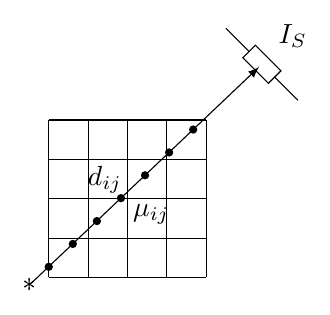
\begin{tikzpicture}[scale=.5, every node/.style={inner sep=-2,outer sep=0}]
		\draw (-2,-2) grid (2,2);
		\draw (60:5) -- (30:5) node[sloped, pos=.5, label={[label distance=10]$I_S$}] (IS) {\fcolorbox{black}{white}{$~~$}};
		\draw[-latex] (-2.5,-2.2) node {\textasteriskcentered} -- (IS);
		\draw[line width=3pt, line cap=round, dash pattern=on 0pt off 4\pgflinewidth] (-2,-1.73) -- (1.925,2);
		\node[label={[label distance=5]135:$d_{ij}$}] at (0,0) {};
		\node[label={[label distance=5]-45:$\mu_{ij}$}] at (0,0) {};
		\end{tikzpicture}
	\end{subfigure}
\end{figure}
\subsection{Lambert-Beer-Gesetz}
\[ I^\text{out} = I^\text{in}\cdot e ^{-\mu\cdot d} \]
\begin{center}
	Schwächungskoeffizienten
\end{center}
%Bild vom Blatt
\begin{align*}
 I_S &= I_0 \cdot e^{ \sum_{\square(i,j) \cap S \neq \emptyset } \mu_{ij}\cdot d_{ij} } \\
 \ln \frac{I_0}{I_S} &= \sum_{\square(i,j)\cap S \neq \emptyset }^{\mu_{ij} \cdot d_{ij} } \\
 I&=\underset{\mathbb{R}^{360. 000. 000 \times 128. 000. 000}}{\underset{\rotatebox{-90}{$\in$}}{D}}\cdot\mu 
\end{align*}
\subsubsection{Inverses Problem}
\paragraph{Gegeben:} Gemessene Intensitäten $I_S$ für alle Strahlen, die die Bildebene treffen für hinreichend viele Aufnahmerichtungen.
\paragraph{Gesucht:} Schwächungskoeffizienten für alle Voxel des zu rekonstruierenden Volumens.
%Bild bzgl. Farbe
\begin{figure}[H]
	\centering
	\begin{tikzpicture}
	\draw[very thin, Gray, dashed] (0,1)--(0,-1);
	\node[draw, square] at (0,0) (c) {$c_0$};
	\draw[-latex] (0,1) -- (c);
	\draw[-latex] (c) -- (0,-1);	
	\end{tikzpicture}
\end{figure}
\[ c^\text{out} = c^\text{in}\cdot\left( 1-\alpha_i \right) + c_i\alpha_i \]
\begin{description}
	\item[$\alpha_i =$]  Deckkraft der Farbe $c_i$
	\item[$1-\alpha_i \hat{=} $] Transparenz
\end{description}
% Stack Bild

\begin{figure}[H]
	\centering
	\begin{tikzpicture}[array/.style={matrix of nodes,nodes={draw, minimum size=7mm},column sep=-\pgflinewidth, nodes in empty cells}]
	\matrix[array] (array) {
		$c_1$\\
		$c_2$\\
		$c_3$\\
		$\vdots$\\
		$c_n$\\	
	};
	%\draw[latex-] (array-1-1.north) -- ++(0, 1);
	\draw[Gray, very thin, dashed] (array-1-1.north) -- (array-5-1.south);
	\draw[-latex] (array-5-1.south) -- ++(0, -1);
	\end{tikzpicture}
\end{figure}
\[ c^\text{out} = \cdot \sum_{i=1}^{n}c_i\alpha_i\prod_{j=i+1}^{n}\left(  1-\alpha_j \right) \]